Le projet \enquote{La couleur~: artefacts, matière et cognition} repose sur plus de 8~000 analyses. Ces dernières se déclinent en une multitude d’informations, de définitions et de commentaires qui sont, en les situant dans un contexte informatique, autant de variables pour un traitement personnalisé de la recherche. Dans le cadre d’une politique d’éditorialisation des données par les utilisateurs, il me semble que proposer la mise en ordre des données dans l’espace est l’une des plus importantes. Les chercheurs ont réuni, au cours des années du projet, des informations précieuses sur les lieux de création des œuvres. Illisibles dans l’immensité d’un fichier~CSV, la représentation de ces données sur une carte permet de produire une distribution dans l’espace de la production artistique et, ainsi, de faciliter l’interprétation avec une approche géographique.\newpage

\section{\indexmot{Leaflet}~: une bibliothèque JavaScript open-source et légère}

La cartographie interactive est un outil précieux pour visualiser et interagir avec des données géographiques de manière dynamique et intuitive. \par
Les données de la base des projets de recherche sont une véritable mine d’informations. Elles n’auraient pu que s’appauvrir en les représentant avec une carte statique classique. Premièrement, cette dernière est contrainte par une image numérique qui prédéfinit une dimension et une résolution, là où la \indexmot{carte interactive} permet des manipulations d’échelles qui évitent les excessives accumulations de données. Ensuite, elle ne permet pas de représenter les variables temporelles, à moins d’être multipliées en autant d’exemplaires que de dates voulues. Enfin, la carte classique ne représente finalement qu’une \indexmot{visualisation} des informations conçue et produite par un cartographe, sans personnalisation possible par l’utilisateur. Sans lister exhaustivement toutes les contraintes – et les limites – d’une telle représentation, ces petits exemples permettent de mesurer la nécessité de réaliser dans le cas présent une cartographie interactive, plus  complexe, mais plus fidèle à la richesse des données de la base.\\\par
Aujourd’hui une \indexmot{carte interactive} peut être réalisée à l’aide d’outils et de plateformes en ligne, comme Google My Maps\footcite{noauthor_google_nodate}, Mapbox\footcite{noauthor_mapbox_nodate} ou encore ArcGIS Online\footcite{noauthor_arcgis_nodate}. Ces plateformes sont gratuites et accessibles à toute personne possédant des rudiments d’informatique, mais elles ne parviennent pas à offrir autant d’avantages et de fonctionnalités que les outils qui nécessitent des connaissances en codage. Ces derniers permettent de personnaliser presque toutes les options de la carte, y compris l’apparence, le comportement et les fonctionnalités. Ils sont réputés avoir une meilleure performance si le nombre de données est amené à être important et, surtout, les outils reposant sur du codage peuvent être plus facilement intégrés dans des applications ou sites Web – comme il en est dans le cas présent. 
Les outils de cartographie sont, pour l’essentiel, des bibliothèques JavaScript, en raison de la simplicité, de l’interactivité et de la performance de ce langage. Il possède également une grande communauté de développeurs qui contribuent à le maintenir à jour et à proposer toujours de nouvelles solutions aux utilisateurs. La communauté JavaScript a développé quelques outils populaires, comme \indexmot{Leaflet}.js\footcite{agafonkin_leaflet_nodate}, OpenLayers\footcite{noauthor_openlayers_nodate}, D3.js\footcite{noauthor_d3_nodate} ou encore Mapbox GL JS. Dans le cadre de ce stage, le choix de la bibliothèque \indexmot{Leaflet}.js, bien qu’elle soit réputée comme étant la plus légère, est apparu comme une évidence. Elle propose, malgré sa simplicité, une large gamme de fonctionnalités de cartographie, notamment en ce qui concerne les marqueurs, les pop-ups, la possibilité de cumuler les filtres ou encore de faire apparaître une barre latérale. Elle propose déjà, en somme, toutes les options qui ont été retenues pour la \indexmot{visualisation} interactive\footnote{Cf. infra.}. De plus, elle est utilisée couramment par le service informatique de l’INHA, service qui hébergera la base Omeka~S du projet\footnote{À titre personnel, la bibliothèque \indexmot{Leaflet} est aussi celle qui me fut enseignée au cours de cette année de master.}. Dans le cadre d’un stage d’une durée de trois mois et avec les conditions énoncées préalablement, il ne m’a pas semblé opportun de continuer l’investigation vers les autres bibliothèques, mais au contraire plus pertinent de chercher à déployer pleinement toutes les potentialités de la bibliothèque \indexmot{Leaflet}. Ainsi, les fonctionnalités plus avancées d’OpenLayers, notamment quant aux tuiles ou aux images raster n’étaient d’aucun intérêt dans le cas présent, D3.js n’est pas nativement conçu pour de la cartographie et aurait complexifié inutilement le travail, tandis que la dernière bibliothèque, Mapbox GL JS, semble plus convenir à un autre public que celui de chercheurs au regard de l’éditorialisation à venir.\\\par
À la date du 18 mai 2023, \indexmot{Leaflet} est à sa version 1.9.4\footnote{Pour notre part, nous avons réalisé le travail à partir de la version 1.8.0.}. La bibliothèque est déposée et peut-être librement téléchargée sur la plateforme GitHub~–~elle pèse seulement 42~ko de JS. Son premier développeur, l’Ukrainien Vladimir Agafonkin, s’est entouré depuis une dizaine d’années d’une petite équipe qui veille au maintien de \indexmot{Leaflet}. La bibliothèque répond ainsi aux innovations du web et aux nouveaux besoins des utilisateurs. Pour ces derniers, les développeurs déposent à l’adresse https://leafletjs.com des tutoriels et une riche documentation qui apportent une réponse à la plupart des questions et des difficultés rencontrées.\par
Une fois téléchargé, le code se divise en trois fichiers et un dossier\footcite{agafonkin_leaflet_nodate}~: 
\begin{itemize}
	\item \texttt{leaflet.js}~: il s’agit du code minifié\footnote{En programmation, minifier signifie réduire la taille du code.}
	\item \texttt{leaflet-src.js}~: le code non-minifié cette fois-ci, ce qui peut permettre un débogage
	\item \texttt{leaflet.css}~: la feuille de style
	\item \texttt{images}~: un dossier contenant les images référencées par le fichier précédent\\
\end{itemize}

Cet ensemble doit être décompressé et placé dans le répertoire du site web. Sur la page HTML, il suffit d’ajouter ces deux lignes pour créer le lien avec la bibliothèque \indexmot{Leaflet}~:\par
<link rel="stylesheet" href="/chemin/vers/le/fichier/leaflet.css" />\par
<script src="/chemin/vers/le/fichier/leaflet.js"></script> \\\par

Les fichiers JavaScript sont alors correctement liés à la page~HTML qui permet de visualiser et déployer la carte sur le site web. Avant de débuter le traitement de la donnée, il convient de poursuivre le travail préparatoire sur les objectifs de la \indexmot{visualisation} et de définir, avec une plus grande précision, les attendus de l’éditorialisation.\newpage

\section{Éditorialiser une base de données avec une cartographie interactive}

La constitution de la base de données par les chercheurs du projet, notamment à partir des \indexmot{thésaurus}, permet d’avoir à disposition des variables qui seront à l’origine de l’éditorialisation. Concrètement, il s’agit dans le cadre d’une cartographie interactive de réaliser le choix d’un ou de plusieurs filtres qui s’appuient sur des clefs, représentées par des colonnes dans les fichiers~CSV, et de porter la sélection sur les valeurs associées, limitées raisonnablement par le \indexmot{thésaurus}. À titre d’exemple, que ce soit pour la base materiality88 ou celle 89, au sein de la colonne \enquote{schema:color} qui représente les couleurs identifiées au moment de l’analyse, le filtre porte sur une sélection entre quinze valeurs~: argenté, beige, blanc, bleu, brun, cuivré, doré, gris, jaune, noir, orange, rose, rouge, vert et violet. Une attribution définie au moment de l’analyse scientifique de l’objet devient ainsi ici une variable qui permet d’éditorialiser~–~de filtrer~–~le résultat pour l’utilisateur.\par
La cartographie interactive est une \indexmot{visualisation} parfaitement adaptée à ce processus de sélection, de désélection et de combinaison de filtres. À la manière des cartes statiques qui laissent une place aux légendes, celles interactives permettent de faire apparaître au plus près les besoins en information et en usage pour l’utilisateur. Elles prennent la forme de quadrilatères équiangles pouvant être disposés selon les souhaits du cartographe. Dans notre cas présent, l’éditorialisation se réalise à partir de quatre filtres, qui peuvent tous s’additionner afin d’affiner la recherche.\\\par
La \indexmot{visualisation} a pour objectif de traduire la circulation et l’utilisation des matériaux de couleur dans la fabrique des enluminures et des panneaux peints sur plus d’un millénaire. C’est une \indexmot{visualisation} qui est non seulement géographique, mais également chronologique. Elle repose ainsi sur quatre variables présentes dans les bases de données~: le matériau (schema:material), la couleur obtenue (schema:color), la localisation (schema:geo) et la date de création (crm:P4\_has\_time-span). Toutes les autres informations présentes dans les bases servent à enrichir les informations proposées par les résultats du filtre, mais elles ne constituent pas les pivots de l’éditorialisation.\par
La première option à la disposition de l’utilisateur émane d’une demande des responsables du projet. Madame Charlotte Denoël, responsable du projet \enquote{La couleur~: artefacts, matière et cognition}, et madame Sigrid Mirabaud, responsable du programme \enquote{La fabrique matérielle du visuel}, souhaitent laisser le choix entre une navigation qui réunirait les deux projets et une autre, qui porterait exclusivement sur l’un d’entre eux. Si les deux projets sont réunis sur la plateforme Omeka~S en raison de leur synergie, ils doivent pouvoir être individualisés à la demande. Ainsi, il convient d’insérer un filtre qui permet la bascule d’un projet à l’autre en première option, tout en proposant leur réunion~–~choix initialisé par défaut.\par

\begin{figure}[H]
	\centering
    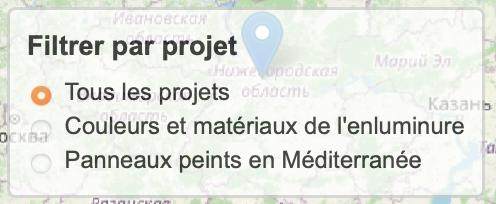
\includegraphics[scale=0.4]{./textes/chap2/filtre-projet.jpg}
	\caption{Filtrer par projet sur la carte}
	\label{fig:info}
\end{figure}

Afin de visualiser l’évolution dans le temps des données, le filtre sur les dates de création est sous la forme d’une jauge. Cette dernière, plus intuitive, est plus à même d’offrir une interaction fluide à l’utilisateur, qui n’a qu’à faire glisser le curseur pour sélectionner une année spécifique. Quant à la granularité de la jauge, les deux bases de données couvrant plus d’un millénaire, j’ai décidé de réaliser une sélection par décennie plutôt que par années. Ce choix doit rendre plus aisé les tendances sur la carte, par une apparition plus fréquente des données. De plus, ce filtre n’est pas, en quelque sorte, \enquote{excluant}, mais au contraire inclut et ajoute progressivement de la donnée à la carte~: le filtre ne représente pas seulement une décennie, mais additionne les créations de ces dernières à celles préexistantes. Ainsi, si nous déplaçons le curseur sur l’année 1060, les manuscrits créent au cours de la décennie s’ajouteront à ceux antérieurs, sans les remplacer. Il me semble que c’est ici proposer une vision plus globale d’un contexte de production, en ne l’isolant pas des dynamiques passées.\par

\begin{figure}[H]
	\centering
	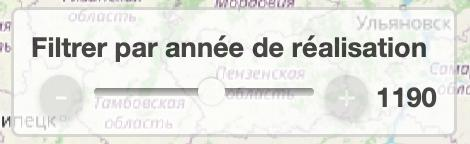
\includegraphics[scale=0.3]{./textes/chap2/filtre-annee.jpg}
	\caption{Filtrer par année sur la carte}
	\label{fig:info}
\end{figure}

La troisième variable est la plus importante du projet. Elle repose sur l’analyse des matériaux et sur leur ontologie. Que ce soit pour la base materiality88 ou celle 89, ces données sont entrées au sein de l’entité \enquote{schema:material}. Fruit d’un long travail, elles reflètent aussi la difficulté de la coordination et de la description manuelle sur un tel corpus. Un script Python révèle qu’à la date du 15~mai 2024, lors d’un travail de normalisation encore en cours, l’entité \enquote{schema:material} possédait 258~valeurs différentes, loin du \indexmot{thésaurus} constitué. Des erreurs d’écriture, plus que de choix, expliquent le résultat~–~nous le remarquons notamment par la présence d’apostrophes qui déprécie l’uniformité\footnote{On rencontre ainsi 1050 occurrences de \enquote{blanc de plomb}, 12 de \enquote{blanc de plomb’} et 10 de \enquote{‘blanc de plomb}.}. De ce fait, un filtre reposant sur une simple sélection n’est pas envisageable. Je propose, pour le choix du matériau, un champ de recherche avec de l’auto-complétion afin de guider l’utilisateur parmi toutes les valeurs~–~l’ordre de la valeur recherchée n’a pas d’importance et le filtre peut être nettoyé à tout moment.\par

\begin{figure}[H]
	\centering
	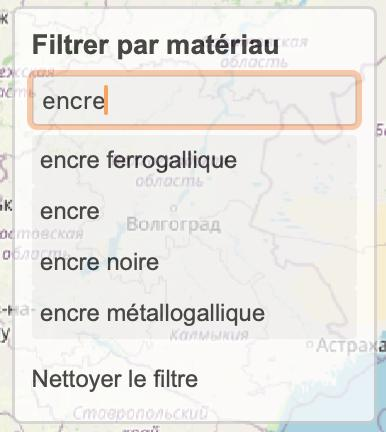
\includegraphics[scale=0.3]{./textes/chap2/filtre-materiaux.jpg}
	\caption{Filtrer par matériau sur la carte}
	\label{fig:info}
\end{figure}

Le dernier et quatrième filtre visible sur la carte porte sur les couleurs. Il semble utile de faire apparaître la concordance ou, au contraire, la discordance de cette variable avec la précédente. Le cumul de ces deux filtres fait ainsi apparaître un maintien ou une disparition de marqueurs que les chercheurs pourront interpréter. Cette entité ne reposant que sur quinze valeurs, j’ai opté pour un sélecteur à choix multiples.\par

\begin{figure}[H]
	\centering
	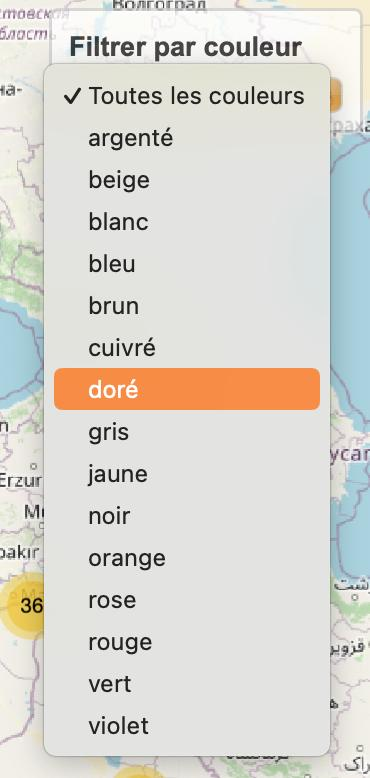
\includegraphics[scale=0.3]{./textes/chap2/filtre-couleur.jpg}
	\caption{Filtrer par couleur sur la carte}
	\label{fig:info}
\end{figure}


L’ensemble de la \indexmot{carte interactive} repose la présence de marqueurs, qui représentent la ou les localisations des feuillets analysés. Ces informations sont entrées au sein de l’entité \enquote{schema:geo}. Cette dernière contient des données de coordonnées géographiques, au format \enquote{latitude, longitude}. Un feuillet peut avoir plusieurs localisations possibles, dans le cadre de contexte de production pluriel ou indéterminé. Au lieu de choisir arbitrairement une seule coordonnée, un même feuillet peut apparaître sur la carte à plusieurs reprises~–~à la condition que les localisations soient éloignées d’au moins trois points de coordonnées pour ne pas surcharger inutilement la \indexmot{visualisation}. Ainsi, le \textit{Pentateuque dit d’Ashburnham ou de Tours} apparaît aussi bien en Afrique du nord, en Espagne, en Italie qu’en France\footnote{\textit{Pentateuque dit d’Ashburnham ou de Tours}, Paris, BnF, NAL 2334}. Lorsqu’ils sont en nombre, les marqueurs sont réunis en clusters – ils sont groupés. Ces derniers indiquent par un chiffre ou un nombre le total des feuillets qu’ils contiennent. Par un agrandissement de la carte ou un clic sur le repère, les marqueurs des feuillets apparaissent. Dans l’exemple ci-dessous, un clic sur le cluster vert situé au niveau de la ville de Milan fait apparaître quatre feuillets analysés du \textit{Liber comitis dit Lectionnaire pourpré}\footnote{\textit{Liber comitis dit Lectionnaire pourpré}, Paris, BnF, Latin 9451}.\par

\begin{figure}[H]
	\centering
	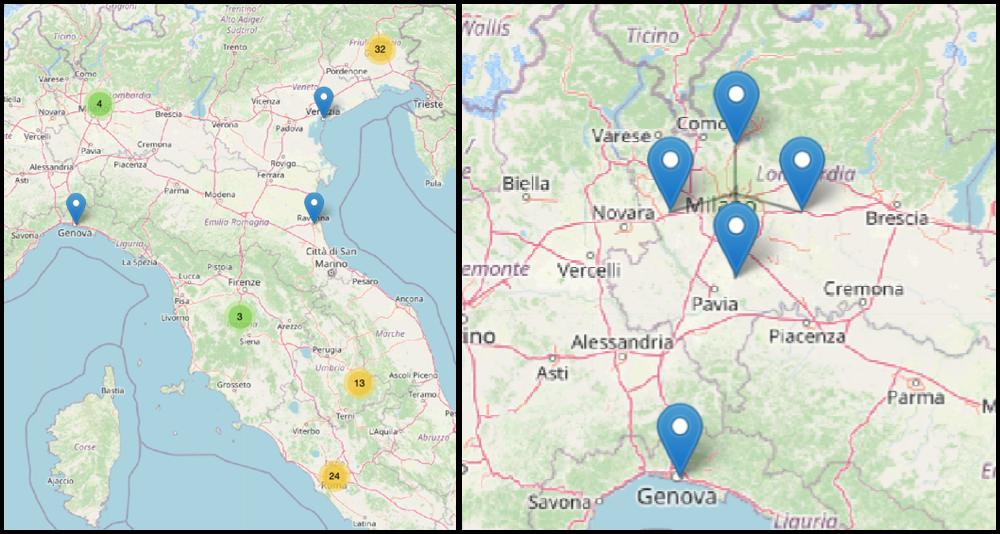
\includegraphics[scale=0.3]{./textes/chap2/localisation.jpg}
	\caption{Marqueurs et clusters}
	\label{fig:info}
\end{figure}

Il est apparu, dans le cadre du projet, qu’il est parfois impossible de proposer une localisation, même indécise, à un manuscrit. Dans ce cas de figure, je prends le parti de définir une localisation par l’absurde afin de faire figurer le marqueur. Situé au large des cotes bretonnes, dans l’Atlantique, le marqueur ne laisse pas de place à une ambiguïté. Une fois le carrousel déployé, il apparaît comme titre du feuillet l’indication \enquote{Lieu de création inconnu}.\\\par
À son lancement, la carte a, par défaut, tous les filtres ouverts et donc tous les marqueurs de représentés. Le filtre \enquote{projet} affiche les résultats sur les deux bases materiality, la date est dans sa dernière décennie, aucun matériau n’est sélectionné, ni aucune couleur définie. L’affichage est centré sur l’Europe et le bassin méditerranéen, où se situent les principaux manuscrits analysés – je crois en l’interactivité de la carte pour que l’utilisateur ait la curiosité de la décentrer et de découvrir des analyses sur des manuscrits produits en d’autres continents. \par

\begin{figure}[H]
	\centering
	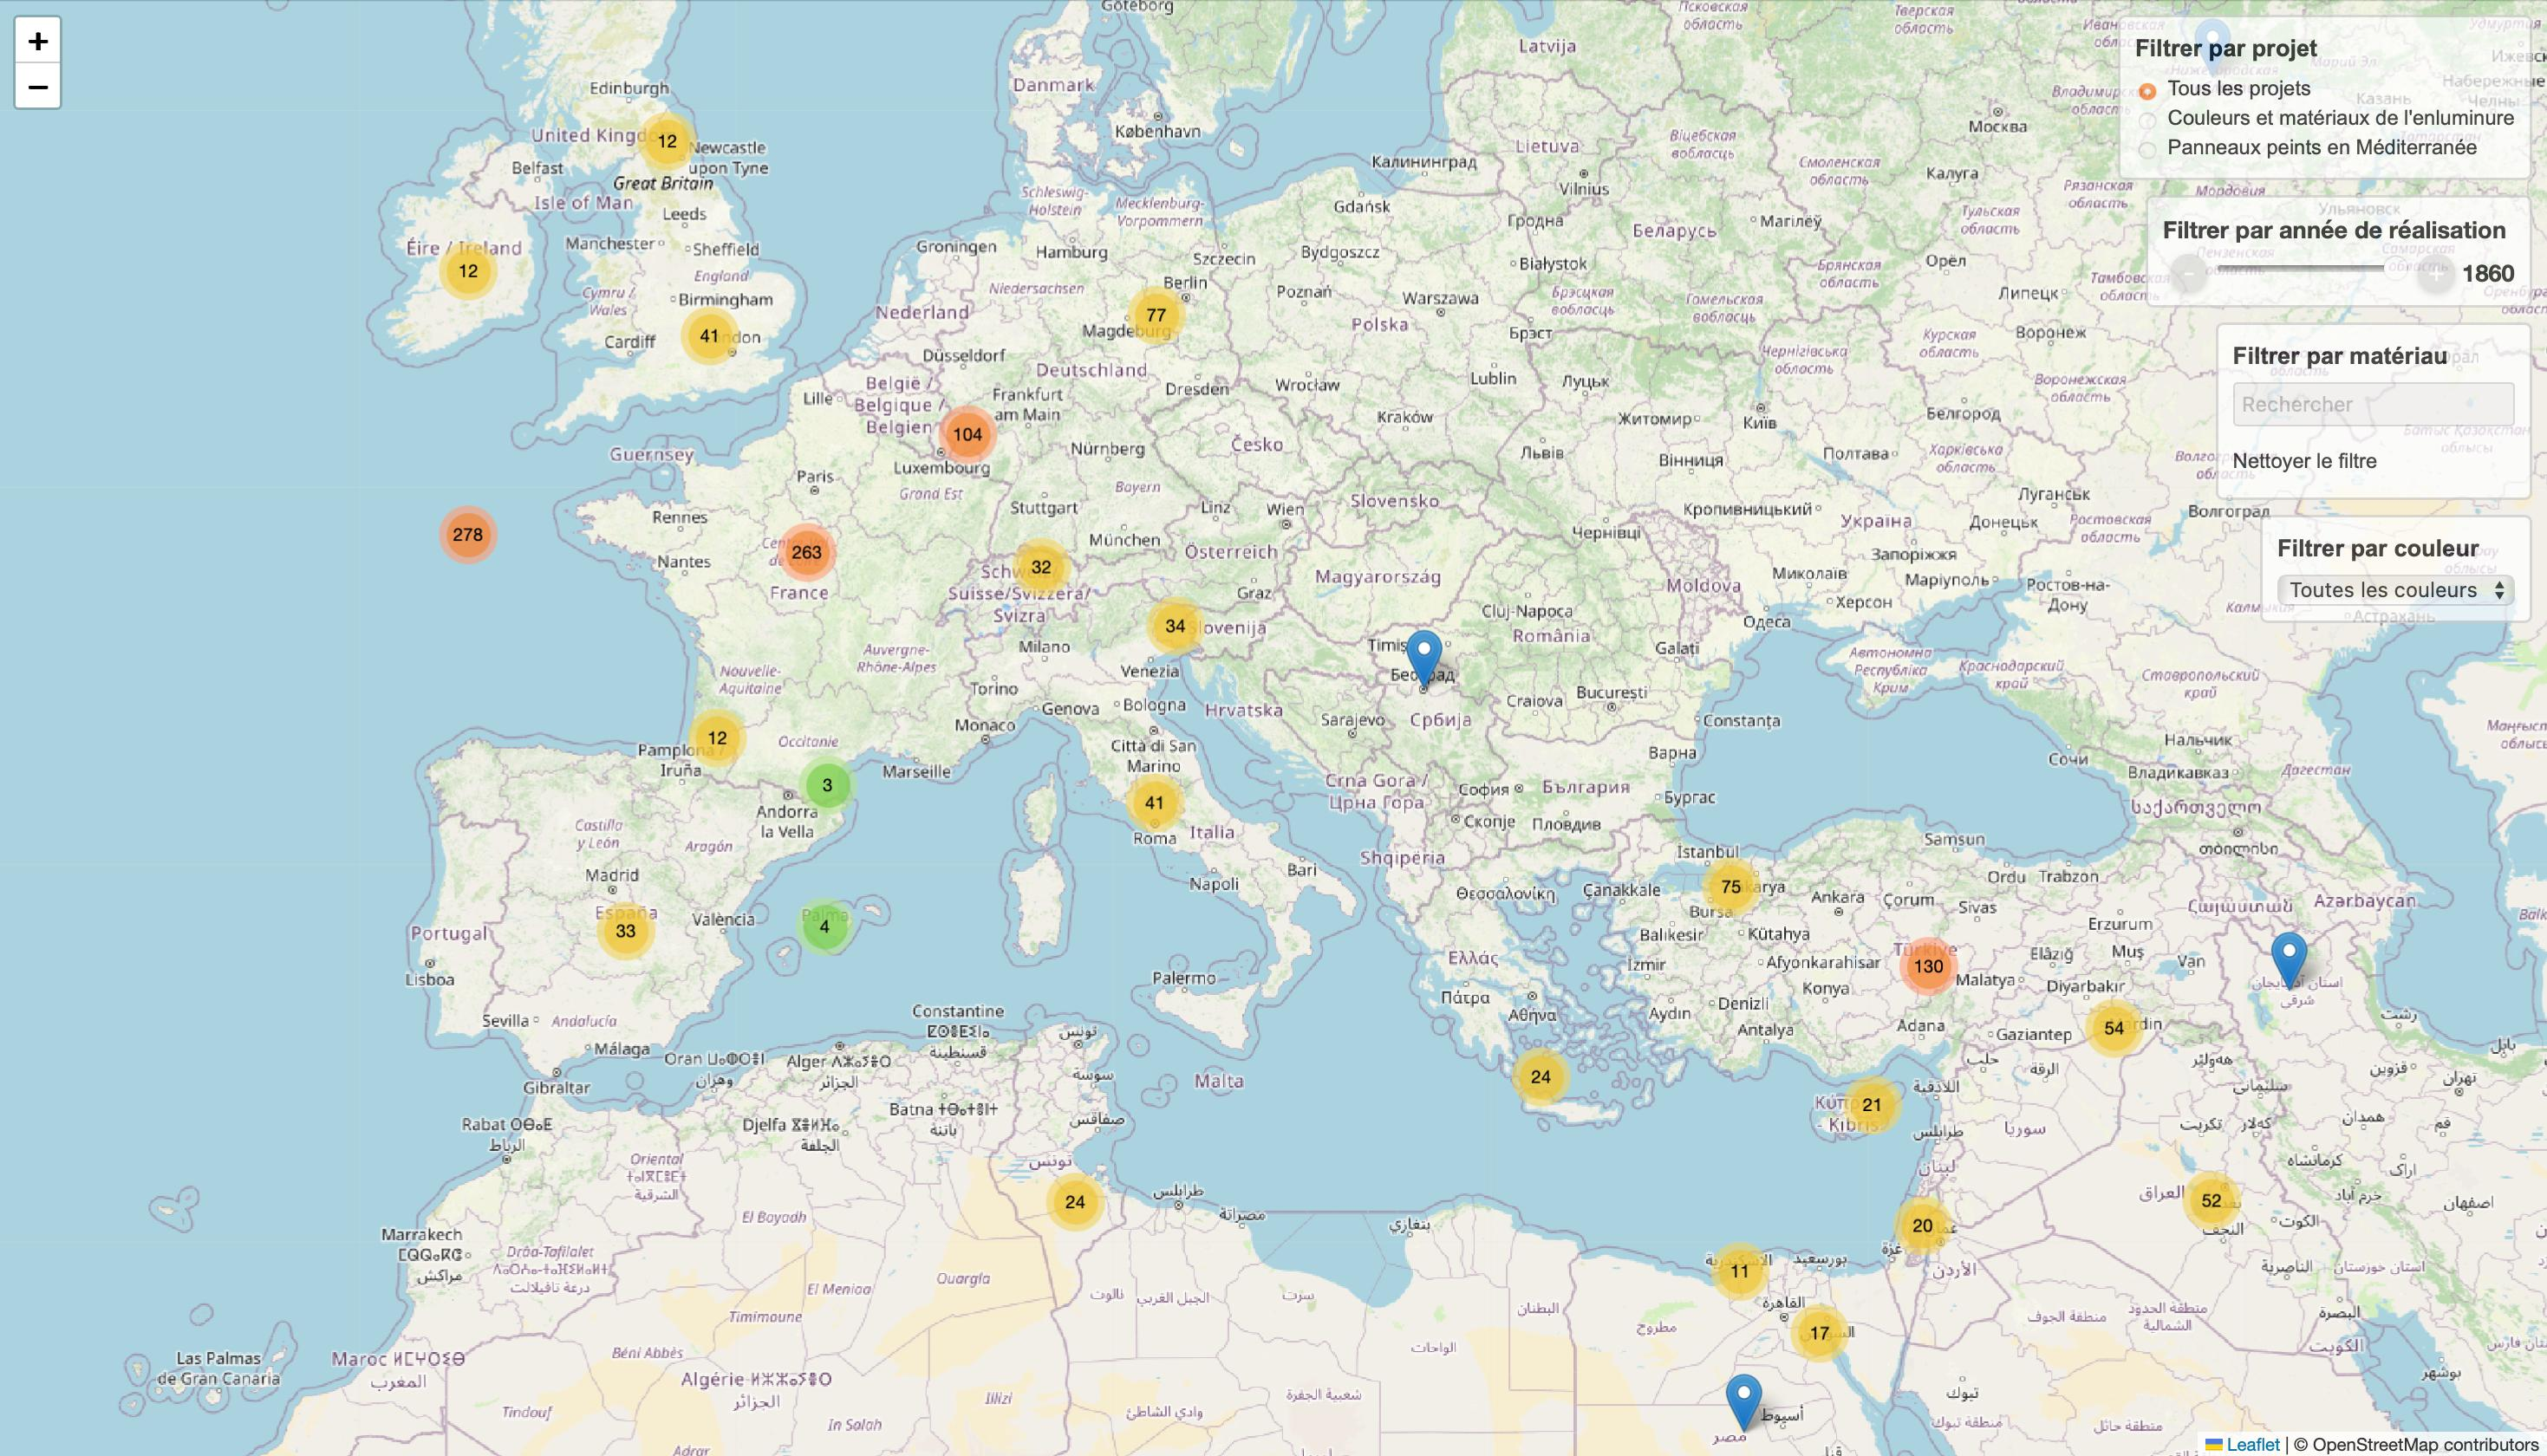
\includegraphics[width=\textwidth]{./textes/chap2/filtre-initialisation.jpg}
	\caption{Initialisation de la carte}
	\label{fig:info}
\end{figure}

Il a été loué précédemment la vertu heuristique du cumul des différents filtres~—~du croisement de variables en interrogeant la base~—~afin de faire apparaître certains résultats dans un contexte géographique et chronologique. La \indexmot{visualisation} ci-dessous, en quatre temps, est insérée à titre d’exemple afin d’apprécier l’efficacité de l’entonnoir produit par les filtres. En partant de la carte initialisée comme précédemment, je définis successivement une base de recherche, les \enquote{Couleurs et matériaux de l’enluminure}, un cadre chronologique avec l’année 1070, la cochenille pour matériau ainsi que la couleur rose. Il apparaît alors vingt-quatre résultats. \textit{Voir la figure 2.7.}\par

\begin{landscape}
	\begin{figure}[ht]
		\centering
		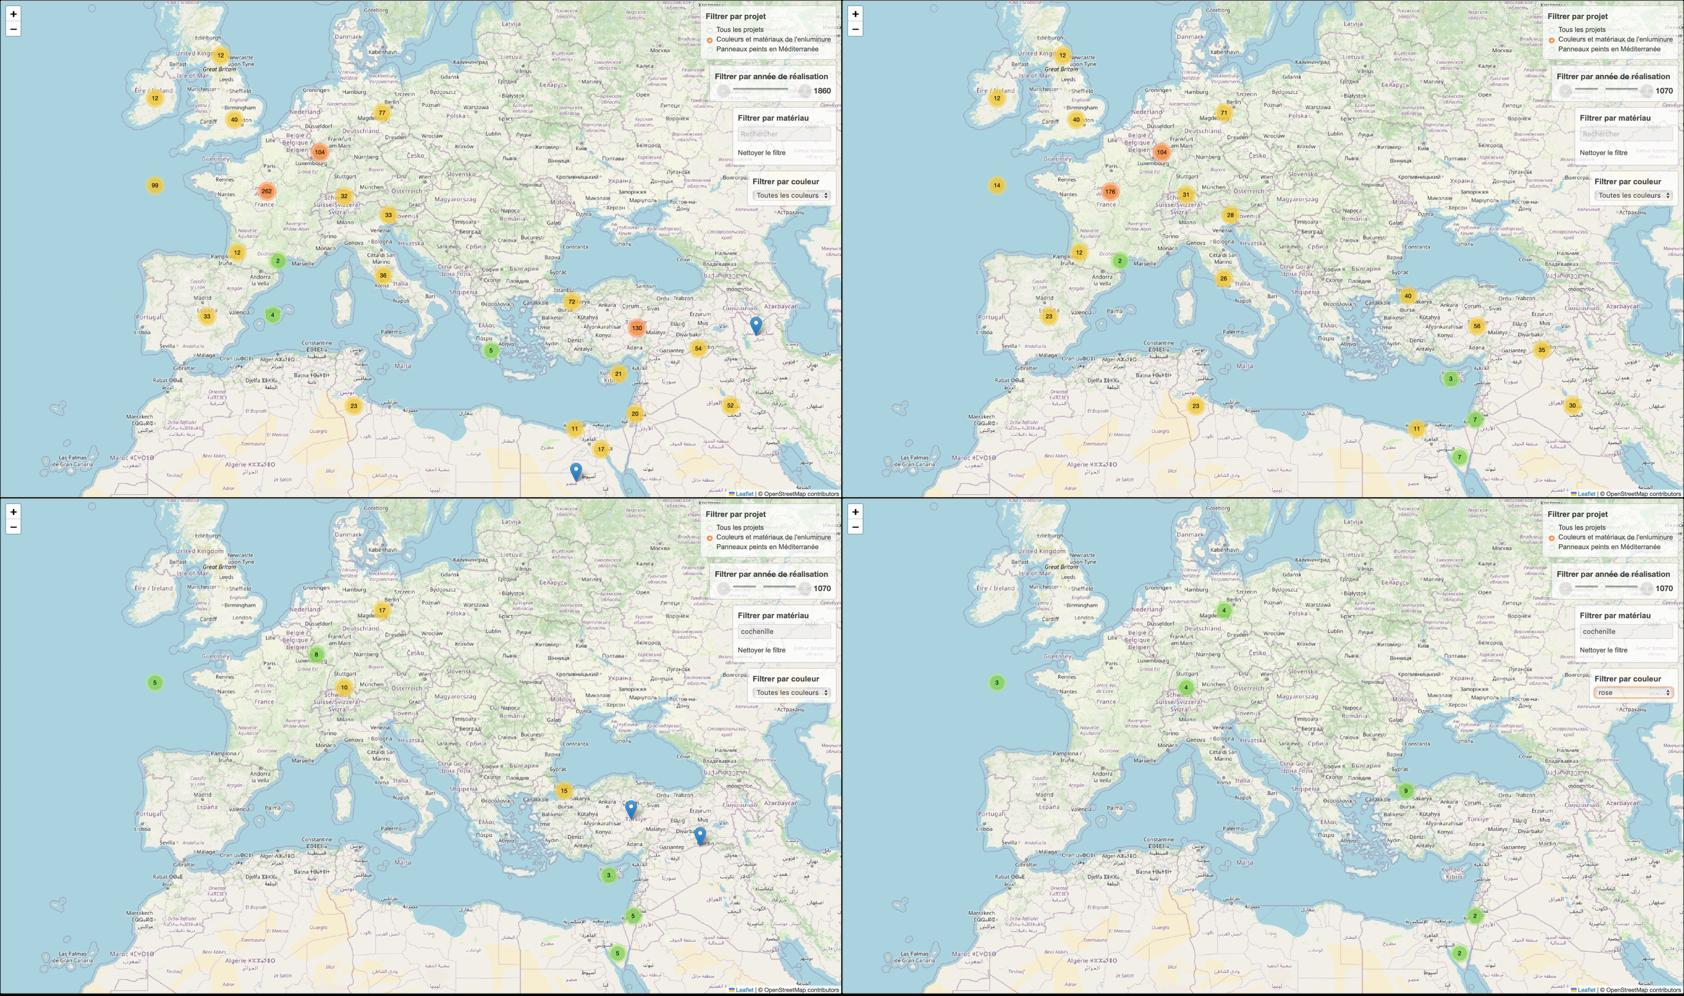
\includegraphics[scale=0.4]{./textes/chap2/filtre-4.jpg}
		\caption{Exemple d'éditorialisation}
		\label{fig:info}
	\end{figure}
\end{landscape}

La lecture des résultats est proposée en trois temps, qui représentent autant de niveaux de détails. Une première info-bulle apparaît lorsqu’un marqueur est survolé par le curseur. Elle reprend l’information entrée dans la colonne \enquote{dcterms:title} et informe sur le titre du manuscrit, sa cote, le nom du feuillet et son numéro. Ce survole rapide accélère le temps de recherche lorsque l’utilisateur est à la recherche d’un feuillet ou d’un manuscrit précis.\textit{Voir la figure 2.8.}\par

Ensuite, un clic permet de déployer un carrousel qui contient les données essentielles sur le feuillet~: une reprise de la colonne \enquote{dcterms:title} comme titre, suivie de l’appel à une image \indexmot{IIIF}~–~image qui peut être agrandie en haute résolution par un nouveau clic. Le carrousel permet une navigation entre les différentes analyses réalisées sur le feuillet. On y trouve ainsi la caractéristique, le motif, la technique, la couleur ainsi que le matériau. \textit{Voir les figures 2.9 et 2.10.}\par


\begin{landscape}
	\begin{figure}[p]
		\centering
		\centering
		\begin{minipage}{0.65\linewidth} % Trois images à gauche
			\centering
			\begin{minipage}{\linewidth}
				\centering
				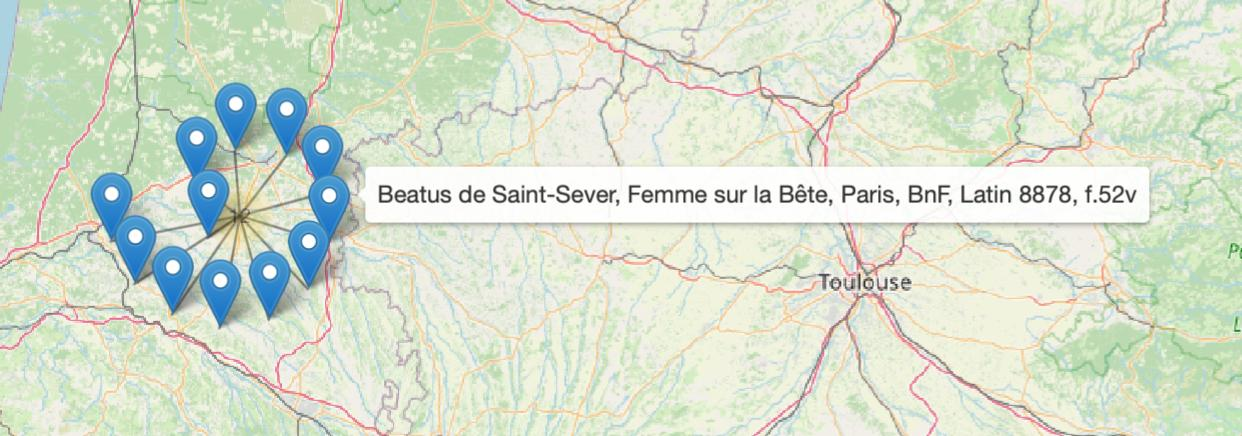
\includegraphics[scale=0.15]{./textes/chap2/info-bulle.jpg}
				\captionof{figure}{Une info-bulle avec les premières informations}
				\label{fig:info1}
			\end{minipage}
			\par\bigskip
			\begin{minipage}{\linewidth}
				\centering
				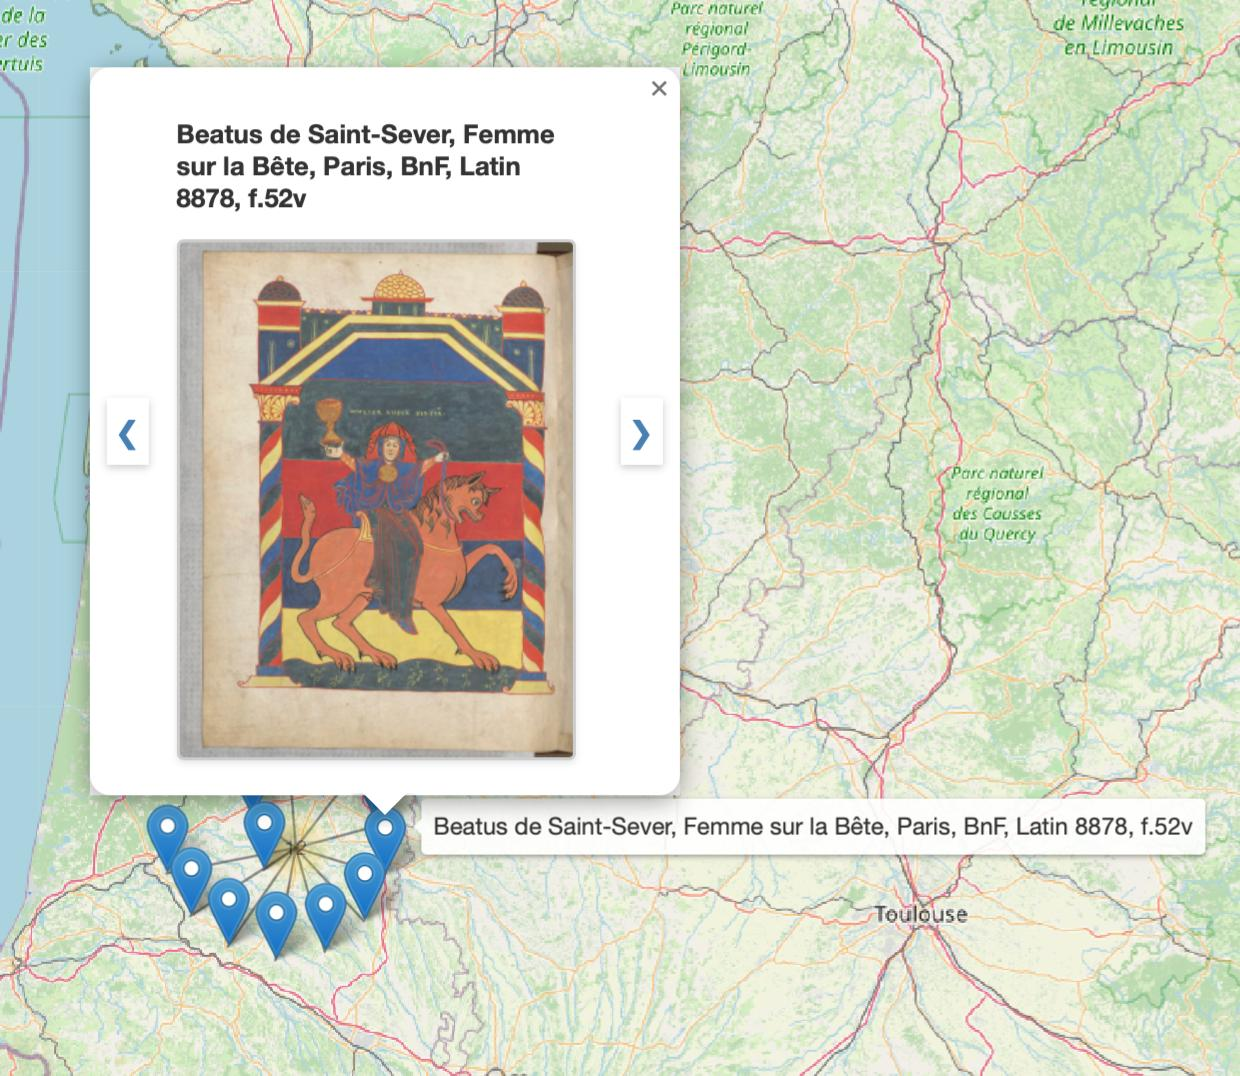
\includegraphics[scale=0.15]{./textes/chap2/carrousel-1.jpg}
				\captionof{figure}{Une image du carrousel}
				\label{fig:carrousel1}
			\end{minipage}
			\par\bigskip
			\begin{minipage}{\linewidth}
				\centering
				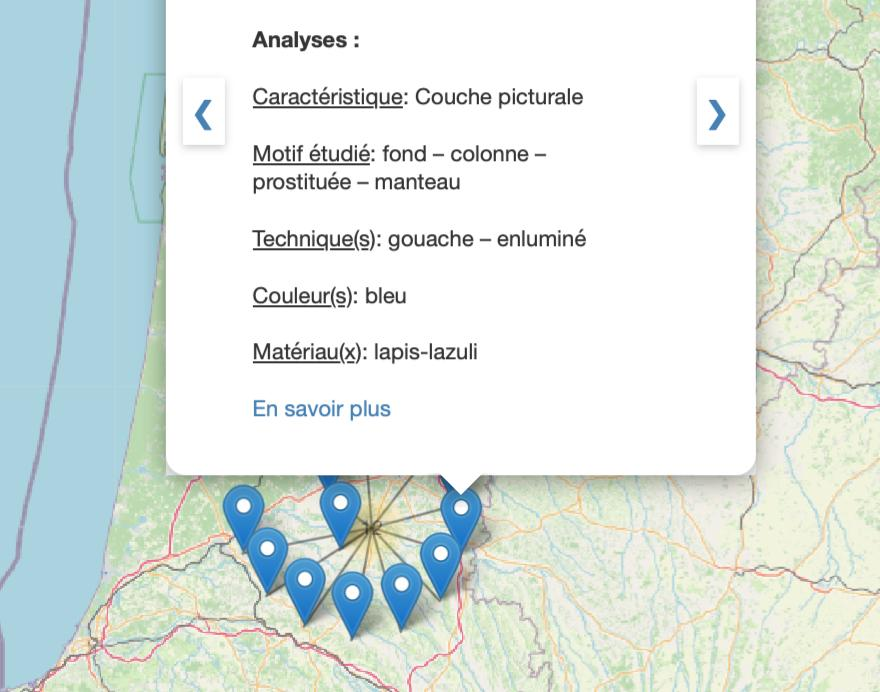
\includegraphics[scale=0.2]{./textes/chap2/carrousel-2.jpg}
				\captionof{figure}{Un descriptif du carrousel}
				\label{fig:carrousel2}
			\end{minipage}
		\end{minipage}\hfill
		\begin{minipage}{0.3\linewidth} % Une image à droite
			\centering
			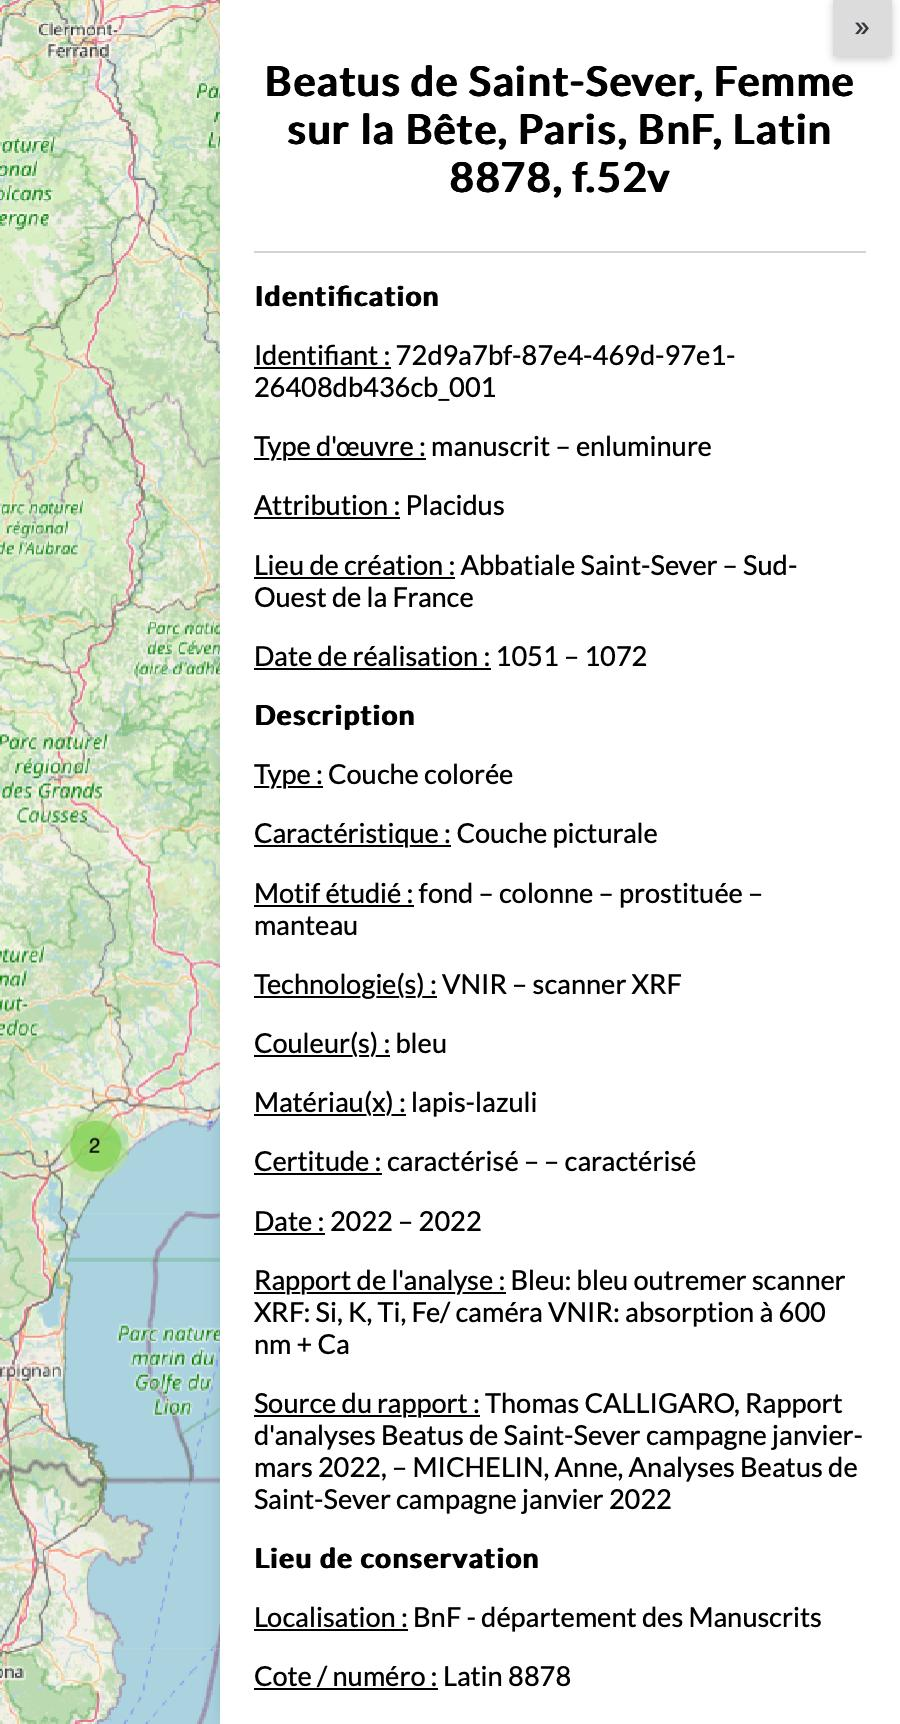
\includegraphics[scale=0.25]{./textes/chap2/slidebar.jpg}
			\caption{Une barre latérale avec la totalité des informations}
			\label{fig:info2}
		\end{minipage}
	\end{figure}
\end{landscape}

Lorsque l’utilisateur trouve le feuillet qui l’intéresse, il peut faire apparaître une barre latérale qui reprend et complète les informations présentes. Il apparaît alors le lieu de création, une éventuelle attribution, d’avantage de détails sur l’analyse, avec notamment les références nécessaires pour la citer, ainsi que des informations sur la conservation actuelle. \textit{Voir la figure 2.11.}\par

La \indexmot{carte interactive} est ainsi le reflet de la richesse du travail réalisé sur les deux bases de données. Elle reprend, d’une façon ordonnée et hiérarchique, toutes les informations essentielles qu’elles contiennent. Si la \indexmot{visualisation} repose sur plus de 8~000 lignes de CSV, elle permet aussi d’individualiser chacune d’entre elles~: le feuillet est représenté dans le travail global du projet de recherche, mais les informations détaillées qui le concernent sont présentes également. La \indexmot{carte interactive} est tout autant une synthèse qu’une analyse. Une synthèse en ce qu’elle propose une vue d’ensemble et cohérente du travail des chercheurs~–~elle est un résumé visuel~; elle est une analyse lorsqu’elle décompose les résultats en fournissant toutes les informations nécessaires pour comprendre les matériaux et les couleurs et que l’utilisateur peut les filtrer selon ses préférences. Pour ce faire, le code doit permettre des allers-retours, des personnalisations, et une exploration plus ou moins profonde des fichiers CSV qui révèlent progressivement les différents niveaux de détail de la recherche. \newpage

\section{Préparer les données}

L’écriture du code se fait sur Visual Studio Code, un éditeur développé par Microsoft pour Windows, Linux et macOS\footcite{noauthor_visual_nodate}. Actuellement dans sa version 1.90.0, cet éditeur inclue une prise en charge du débogage, une mise en évidence de la syntaxe, parfois une complétion intelligente du code et, point important dans le cas présent, une intégration de Git . Ce dernier aspect est essentiel lorsque le code écrit repose sur des essais qui sont validés, corrigés ou invalidés. Le travail sur une bibliothèque de cartographie interactive est dans la pratique essentiellement empirique et ne nécessite que ponctuellement de s’aventurer dans les pages de la documentation. Des lignes de code sont écrites, on observe un résultat, on les corrige par petites touches ou retranchements jusqu’à ce que le résultat finalement soit satisfaisant et conforme à l’attendu. La possibilité de réaliser des allers-retours est ainsi essentiel, tout comme la celle de pouvoir comparer différentes étapes et les réunir le cas échéant. De ce fait, l’implémentation de Git Lens\footcite{noauthor_gitlens_nodate} et de Git Graph\footcite{noauthor_git_nodate} à VSCode, deux extensions qui facilitent l’expérience du codage, notamment par des \indexmot{visualisation}s claires de l’historique des commits, est un plus. Live Server\footcite{noauthor_live_nodate} est la troisième extension nécessaire, elle permet de lancer un serveur web local pour prévisualiser les pages web en temps réel. Chaque modification apportée dans le code est alors aussitôt visible sur la \indexmot{carte interactive}.\\\par
Une fois ces paramétrages effectués, le travail avec la bibliothèque \indexmot{Leaflet} peut commencer. Je ne présenterai ici que les lignes directrices qui conduisent à la \indexmot{visualisation} obtenue, pas une reprise détaillée de chaque ligne du code. Ce dernier est commenté et est disponible à l’adresse \url{https://github.com/TheoBurnel/Stage.git} le cas échéant.\par
Dans un premier temps, le travail repose sur quatre fichiers CSV fournis par l’INHA qui reprennent toutes les informations entrées dans Agorha par les porteurs du projet~: artwork88, artwork89, materiality88 et materiality89. La \indexmot{visualisation} est souhaitée à partir des feuillets analysés, et non pas des manuscrits. De ce fait, l’essentiel des données repose sur les deux derniers fichiers, les premiers n’étant présents dans mon code que pour la récupération des images des feuillets en question~–~la colonne \enquote{dcterms:image} qui contient les liens des images n’existe pas dans les fichiers materiality88 et 89. Un code Python permet de n’extraire de ces CSV que l’identifiant du feuillet ainsi que le lien vers son image, une liaison par l’identifiant peut alors se faire avec les deux autres bases CSV\footnote{Voir le code \enquote{ images.py}, puis \enquote{lien.py} à l’adresse \url{https://github.com/TheoBurnel/Stage/tree/9c0841f622f3f39d51615e129507a4bf9a2abaf9/leaflet/python}}. Concernant les deux CSV principaux, le code Python « nettoyage » me permet d’isoler les identifiants des feuillets, de sélectionner les coordonnées voulues et au bon format, de supprimer d’éventuels doublons et enfin de les réunir en un seul fichier\footnote{Voir le code à l’adresse \url{https://github.com/TheoBurnel/Stage/tree/9c0841f622f3f39d51615e129507a4bf9a2abaf9/leaflet/python}}. Une fois la concaténation faite avec les images présentes dans les fichiers artwork, j’obtiens un tableau de 10701~lignes pour 37~colonnes, soit 395~937~entrées pour l’analyse. La cartographie est bien le reflet d’une grande étude, non seulement qualitative, mais également quantitative.\par
Après la phase préparatoire et avant de passer au code JavaScript, il est nécessaire de transformer le fichier~CSV obtenu en données JSON. À ce moment, le langage Python est encore nécessaire. Il l’est dans un premier temps pour donner une structure appropriée au fichier de sortie~–~un fichier .json, mais il l’est également pour la définition d’une entité \enquote{parent} et d’une \enquote{enfant} qui serviront à la réalisation du carrousel de la carte. Puisque la \indexmot{visualisation} repose sur les feuillets, il convient de définir les valeurs de la colonne \enquote{crm:P106i\_forms\_part\_of} comme des parents des valeurs présentes dans celle \enquote{dcterms:title} où se trouvent les analysées réalisées. En d’autres termes, un feuillet qui a pour valeur~–~identifiant~– \enquote{ 02389266-ee27-48ea-be1e-0b40e5e0144e} sert de pivot~–~de socle à la rotation du carrousel~–~aux analyses \enquote{ 02389266-ee27-48ea-be1e-0b40e5e0144e\_001}, \enquote{02389266-ee27-48ea-be1e-0b40e5e0144e\_002}, \enquote{ 02389266-ee27-48ea-be1e-0b40e5e0144e\_003}, etc. Cette attribution faite, il possible d’encoder le tableau au format idoine pour débuter le travail de cartographie\footnote{Un exemple de résultat pour une analyse est également proposée à l’annexe~2.}.\newpage

\section{Coder la bibliothèque JavaScript \indexmot{Leaflet}}

Le code repose sur un fichier~JSON d’un peu plus de sept cents lignes. Ne pouvant le détailler ici, je me propose de me concentrer sur le traitement de l’entité \enquote{schema:material}, qui concerne les entrées sur les matériaux. Sa présentation permet de montrer un travail réalisé sur une entité de première importance, mais également un modèle de création de filtre avec la bibliothèque \indexmot{Leaflet}.\par
Après les premières lignes qui initialisent la carte, chargent les tuiles et instaurent les principes des clusters pour les marqueurs, il convient de reprendre le travail sur la définition des entités parent ou enfant. Le code est le suivant~:\par
\begin{lstlisting}
	// Fonction pour vérifier si c'est un parent (adulte)
	function isParent(titre) {
		return titre && titre.trim() !== ''; // Considérer comme parent si le titre n'est pas vide
	}
	
	// Fonction pour récupérer les enfants par parent
	function getChildrenByParent(parent) {
		var children = [];
		// Logique pour récupérer les enfants
		geojson_RAMA.features.forEach(function (feature) {
			if (feature.properties.Parent === parent) {
				children.push({
					// Exemple pour récupérer la valeur des matériaux
					// Il faut fonctionner de façon similaire pour toutes les autres entrées
					materiaux: feature.properties.Materiaux || '?',
					// etc etc.
				});
			}
		});
		
		return children;
	}
\end{lstlisting}\par
À présent, le socle du carrousel peut être définie sur les entrées du titre, à savoir la colonne \enquote{dcterms:title}, tandis que le défilement se fera sur l’ensemble des enfants récupérés, à savoir les autres colonnes de la même ligne.\par
Le contenu du carrousel tient en quelques lignes~:\par
\begin{lstlisting}
	// Fonction pour créer le contenu du carrousel pour les enfants
	function createCarousel(parent, identifiant) {
		var carouselContent = "<div class='carousel'><div class='carousel-content'>";
		
		var children = getChildrenByParent(parent);
		children.forEach(function (child, index) {
			var displayStyle = index === 0 ? 'block' : 'none';
			
			carouselContent += "<div class='slide' style='display: " + displayStyle + "; padding-left: 30px;'>";
			if (child.coordinates && child.coordinates.length === 2 && child.coordinates[0] === -8 && child.coordinates[1] === 48) {
				carouselContent += "<p><h4><u>Lieu de création inconnu</u></h4></p>";
			}
			carouselContent += "<h3>" + child.titre + "</h3>";
			
			if (child.image && child.image !== '?') {
				carouselContent += "<img id='carousel-image-" + index + "' src='" + child.image + "' onclick='expandImage(this)' />";
			}
			carouselContent += "<p class='carousel-legend'>Identifiant de la photo :<br>" + child.name + "</p>";
			
			carouselContent += "<p><h4>Analyses :</h4></p>";
			// Jusqu’à présent, le carrousel a un titre, une valeur par défaut pour les lieux de création inconnus, une image téléchargée automatiquement avec une légende et également un paragraphe introduisant les résultats des analyses. Il convient à présent d’y mettre les informations souhaitées. Pour les matériaux : 
			
			if (child.materiaux && child.materiaux !== '?') {
				carouselContent += "<p><u>Matériau(x)</u>: " + child.materiaux + "</p>";
			}
		});
		
		return carouselContent;
	}
\end{lstlisting}\par
Il est en de même pour les autres entrées. Le carrousel se termine par un lien vers la barre latérale, la création des flèches pour le défilement ainsi que la possibilité d’agrandir l’image téléchargée. Les lignes pour la définition du contenu de la barre latérale sont très proches de celles pour la carrousel, il convient simplement de bien veiller à la correspondance entre les éléments parents, autrement dit de faire correspondre les feuillets et les analyses. À la fin du carrousel, le lien est défini par cette ligne~:
\begin{lstlisting}
	 carouselContent += "<p class='slidebar-link' onclick='showSlidebar(" + JSON.stringify(child) + ")'>En savoir plus</p>";
\end{lstlisting}\par
Ce qui permet de récupérer les informations dans la barre latérale~:
\begin{lstlisting}
	// Fonction pour afficher la slidebar avec les détails de l'élément sélectionné
	function showSlidebar(child) {
		var slidebar = document.createElement('div');
		slidebar.className = 'slidebar';
		
		// Création du contenu HTML de la slidebar en vérifiant les valeurs
		var slidebarContent = `
		<div class="slidebar-content">
		<button class="close-btn" onclick="hideSlidebar()">&raquo;</button>
		<div class="slidebar-header">`;
\end{lstlisting}\par
Puis d’appeler le contenu, avec l’exemple des matériaux~:
\begin{lstlisting}
	if (child.materiaux && child.materiaux !== '?') {
		slidebarContent += `<p><u>Matériau(x) :</u> ${child.materiaux}</p>`;
	}
\end{lstlisting}\par
L’entité \enquote{schema:material}, nous l’avons vu, est également à la source d’un filtre. Ses deux cent cinquante-huit valeurs différentes doivent constituer des variables sur lesquelles il est possible de réaliser une sélection. Afin de pouvoir permettre une éventuelle mise à jour de l’ontologie sur les matériaux, notamment sur les corrections que nous avons évoquées précédemment, les valeurs ne sont pas écrites en dur dans le code. Elles sont appelées pour être directement retranscrites dans un ensemble qui les stocke. À cette occasion, les données sont aussi partiellement nettoyées de leurs défauts. Ensuite, un tableau est créé, dans lequel les résultats individualisés sont à la fois clef et valeur pour le filtrage. Une fois ces données prêtes, l’ajout du panneau de contrôle, l’auto-complétion, ainsi que nettoyage du filtre se codent sans difficulté. Plus complexes, en revanche, sont le paramétrage du filtre et sa liaison aux trois autres.\par
Pour le premier, la solution est de réaliser des méthodes \enquote{querySelector} sur les valeurs rassemblées. \enquote{querySelectorAll} renvoie à une liste statique, ici l’ensemble des entrées du tableau~; elle permet ainsi d’initialiser le filtre au lancement de la carte, tout comme de nettoyer le filtre. De son côté, \enquote{querySelector} renvoie l’élément qui correspond à l’entrée voulue.\par
\begin{lstlisting}
	// Appeler la fonction d'initialisation une fois que le DOM est chargé
	document.addEventListener('DOMContentLoaded', function () {
		initMaterialItems();
	});
	
	// Fonction pour réinitialiser le filtre de recherche de matériau
	function resetMaterialFilter() {
		var materialElements = document.querySelectorAll('.material-item');
		
		// Cacher tous les éléments matériau
		materialElements.forEach(function (element) {
			element.style.display = 'none';
		});
	}
	
	// Fonction appelée lors de la sélection d'un matériau dans la liste
	function selectMaterial(material) {
		updateMateriauFilter(material);
		// Réinitialiser le filtre après la sélection d'un matériau
		resetMaterialFilter();
		
		// Sélectionner le champ de recherche
		var searchInput = document.querySelector('input[type="text"][placeholder="Rechercher"]');
		// Mettre à jour la valeur du champ de recherche avec le matériau sélectionné
		if (searchInput) {
			searchInput.value = matériaux[material] || ""; // Utiliser le libellé correspondant à la clé sélectionnée
		}
	}
	
	// Fonction pour nettoyer le filtre de recherche de matériau
	function clearMaterialFilter() {
		// Réinitialiser le champ de recherche
		var searchInput = document.querySelector('input[type="text"][placeholder="Rechercher"]');
		if (searchInput) {
			searchInput.value = ''; // Effacer le texte du champ de recherche
		}
		
		// Réinitialiser et afficher tous les éléments matériau
		var materialElements = document.querySelectorAll('.material-item');
		materialElements.forEach(function (element) {
			element.style.display = 'block'; // Afficher tous les éléments matériau
		});
	}
	
	// Ajouter le contrôle de recherche à la carte
	controlSelect.addTo(map);
\end{lstlisting}\par
Mais pour que ce paramètre fonctionne de manière synchronisée avec les autres, il faut que les filtres sur les projets, la décennie et la couleur soient mis à jour au moment de son lancement. Pour le filtre matière, la fonction tient en trois lignes~–~il convient de faire de même pour les autres filtres~: 
\begin{lstlisting}
	// Fonction pour mettre à jour le filtre par matériau
	function updateMateriauFilter(value) {
		currentMateriauFilter = value;
		filterMarkersByDateTypeAndColorAndMateriau(currentYearFilter, currentMateriauFilter, currentColorFilter, currentBaseFilter);
	}
\end{lstlisting}\par
Dernière partie du code, les marqueurs sont la finalisation de tout ce qui précède. Ils font apparaître sur la \indexmot{carte interactive} les résultats et ils communiquent les informations et les données correspondantes. Ce sont les marqueurs, d’abord réunis en cluster, qui contiennent dans un premier temps l’info-bulle, puis le carrousel et enfin la barre latérale. À chaque étape de la \indexmot{visualisation}, ils délivrent ainsi les renseignements recherchés par l’utilisateur.\par
\begin{lstlisting}
	// FONCTION POUR RÉCUPÉRER LES DONNÉES
	// Fonction pour filtrer les marqueurs par année, matériau, couleur et filtre de base
	function filterMarkersByDateTypeAndColorAndMateriau(yearFilter, materiauFilter, colorFilter, baseFilter) {
		// Nettoie les anciens marqueurs de la carte
		markers.clearLayers();
		
		// Utilisation d'un objet pour suivre les marqueurs parent déjà ajoutés
		var parentMarkers = {};
		
		// Parcours de chaque entité (feature) dans les données géographiques (geojson)
		geojson_RAMA.features.forEach(function (feature) {
			// Extraction de l'année à partir de la propriété 'Date_filtre' de l'entité
			var dateYear = parseInt(feature.properties.Date_filtre.split("-")[0]);
			// Récupération des autres propriétés de l'entité
			var type = feature.properties.Type;
			var couleur = feature.properties.Couleur;
			var parent = feature.properties.Parent;
			var projet = feature.properties.Projet;
			var titre = feature.properties.Titre;
			
			// Nettoyer la valeur du filtre de base en mettant en minuscule et en supprimant les apostrophes
			var cleanedBaseFilter = baseFilter.toLowerCase().replace(/'/g, '');
			
			// Vérifier si l'entité est un parent en fonction de son identifiant
			if (isParent(feature.properties.Identifiant)) {
				// Appliquer les filtres : année, matériau, couleur et filtre de base
				if (
				dateYear <= yearFilter &&
				(materiauFilter === '' || feature.properties.Materiaux.toLowerCase().includes(materiauFilter.toLowerCase())) &&
				(colorFilter === '' || couleur.toLowerCase().includes(colorFilter.toLowerCase())) &&
				(cleanedBaseFilter === '' || projet.toLowerCase().includes(cleanedBaseFilter))
				) {
					// Vérifier si le parent n'a pas encore été ajouté comme marqueur
					if (!(parent in parentMarkers)) {
						// Récupérer les coordonnées de l'entité pour créer un marqueur \indexmot{Leaflet}
						var coordinates = feature.geometry.coordinates;
						var marker = L.marker([coordinates[1], coordinates[0]]);
						var identifiant = feature.properties.Identifiant;
						
						// Créer le contenu de la fenêtre contextuelle (popup) à afficher
						var popupContent = createCarousel(parent, identifiant);
						
						// Créer et attacher une infobulle (tooltip) au marqueur
						var tooltip = L.tooltip().setContent(titre);
						marker.bindTooltip(tooltip);
						
						// Attacher le contenu de la fenêtre contextuelle (popup) au marqueur
						marker.bindPopup(popupContent, {
							maxHeight: 400
						});
						
						marker.on('popupopen', function (e) {
							updatePopupMaxHeight(e.popup); // Mettre à jour la hauteur maximale de la fenêtre contextuelle lors de l'ouverture
						});
						
						marker.on('popupcontentupdate', function (e) {
							updatePopupMaxHeight(e.popup); // Mettre à jour la hauteur maximale de la fenêtre contextuelle lors de la mise à jour du contenu
						});
						
						// Cacher la barre latérale lorsque la fenêtre contextuelle se ferme
						marker.on('popupclose', function () {
							hideSlidebar();
						});
						
						// Ajouter le marqueur à la couche de marqueurs (markers)
						markers.addLayer(marker);
						
						// Marquer le parent comme ayant été ajouté
						parentMarkers[parent] = true;
					}
				}
			}
		});
		
		// Ajouter la couche de marqueurs à la carte
		map.addLayer(markers);
\end{lstlisting}

\newpage

\section{La cartographie interactive et ses biais}

Le chapitre précédent ne propose qu’un aperçu du code pour la réalisation de la \indexmot{carte interactive}. Je me suis restreint à la seule entité des matériaux, soit une seule colonne parmi les trente-sept du tableau obtenues après le prétraitement avec le langage Python. Cependant, le cas des matériaux permet d’avoir un aperçu non seulement sur la récupération des valeurs des entités, mais aussi sur l’encodage d’un filtre. Si l’exercice de la présentation d’un code peut sembler relever d’un aspect purement technique, il me semble que sa compréhension est essentielle en ce qu’il conditionne lui-même l’interprétation.\par
La conception et l’encodage de la cartographie interactive façonnent la manière dont les utilisateurs interagissent avec les données et, par conséquent, comment ils les interprètent. Dans un premier temps, il convient de rappeler que les analyses présentées le sont par feuillet et non par manuscrit. Il existe ainsi, à la lecture de la carte, une surreprésentation des matériaux des manuscrits qui ont le plus de feuillets analysés. En outre, plus de soixante pour cent des analyses proviennent de fonds conservés à la \indexmot{Bibliothèque nationale de France}. \par
Le choix et la présentation des filtres conduisent les utilisateurs à s’intéresser prioritairement aux matériaux, soit en lien avec une \indexmot{chronologie}, soit avec une couleur. Les récurrences de motifs ou de techniques sont partiellement délaissées, du moins renvoyées à des précisions lors du déploiement de la barre latérale. Cependant, je ne pense pas que l’on puisse évoquer un possible biais ici. Il s’agit simplement de faire droit à ce qui est la raison même du projet sur \enquote{La couleur~: artefacts, matière et cognition}, bien que ce dernier ait pu apporter de nouvelles connaissances par la suite, par exemple sur les attributions des œuvres. En revanche, les filtres sur les matériaux et les couleurs ne proposent des \indexmot{visualisation}s que sur une seule sélection au sein de leur ontologie ; là où certains chercheurs auraient pu souhaiter questionner la coexistence de certains matériaux au sein d’un même feuillet\footnote{Il s’agit d’une motivation supplémentaire pour proposer la \indexmot{visualisation} Vikus. Voir le chapitre~3.}.\par
Il n’y a pas de véritable sélection dans le choix de données à inclure ou à exclure. L’affichage en deux temps que permet la \indexmot{carte interactive}, d’abord avec le carrousel, puis avec la barre latérale, permet de retranscrire presque l’intégralité des informations présentes dans les bases materiality88 et 89. Cependant, l’affichage du carrousel conduit bien à une lecture sur les analyses mêmes, tandis que la barre latérale apporte les informations complémentaires sur le manuscrit. En dernier lieu, les marqueurs et les clusters sont neutres dans leur \indexmot{visualisation}. La taille et l’icône ne disent rien, tandis que la couleur vive est réservée logiquement aux clusters avec le plus d’occurences.\newpage

* \\

La \indexmot{carte interactive} ne se limite pas à éditorialiser les données~; elle les organise aussi selon des critères géographiques, rendant ainsi intelligible une base de données complexe. Elle offre une \indexmot{visualisation} claire de la distribution géographique des enluminures et des panneaux peints analysés. Pour les chercheurs, elle facilite une interprétation principalement spatiale des données, tout en servant de moyen de communication auprès d'un public plus large. En permettant une navigation aisée à travers les données, elle permet de découvrir les œuvres dans leur contexte géographique et historique.